\chapter{Game theory}
We now move away from situations where a single agent maximizes their own objective functions in different situations (e.g., individuals picking their consumption bundle to maximize their utility or firms maximizing profits) to models where there are multiple agents. Each agent has an objective function and make choices based on that function. Crucially, one agent's choices could affect the payout to other agents in game theoretic models. That its, they play a ``game" together.

\section{Monopoly}
The canonical monopoly model is usually taught after learning about firm's profit maximization problem, but both this course puts it towards the end together with the game theory content. In a sense, the monopoly model is a game with two players: the monopoly firm and the market. 
\subsection*{Review and extension of the profit maximization problem}
Suppose a firm produces quantity $q$ with cost $C(q)$, we say that it maximizes profits $\pi$ by choosing quantity as follows
\begin{equation}
    \max_q \pi(q) = pq - C(q) \label{gt:originaleq} 
\end{equation}
In chapter three, we assumed that there is a perfectly competitive market our good and the firm is a price taker. One way this could arise is when there are other firms who are also making the same good at price $p$, and if our prices became any higher, customers will substitute to the competitor good and we will sell nothing. The above equation gives us the FOC $p = C'(q)$, or price equals marginal cost.

In a monopoly market, only a single company produces the good and it can set the prices it sell the good at. However, the market demand for the good is not unlimited and is dependent on the price (otherwise we will set prices to infinity). We assume that demand monotonically decreases with price, and thus we can write down the inverse function $p(q)$. This function tells us what price we would have to set in order to sell $q$ units of our good.
\begin{equation}
    \max_q \pi(q) = p(q)q - C(q) \label{gt:monoeq} 
\end{equation}
Which gives us the FOC 
\begin{equation}
    p'(q)q + p(q) = C'(q) \label{gt:monoeqfoc} 
\end{equation}
Which sets marginal cost equal to marginal revenue. Notice that this is exactly the same as the previous case when the effect of quantity on price is zero (i.e., $p'(q) = 0$). We can also rewrite equation \ref{gt:monoeqfoc} as
\begin{equation}
    p\left(1 + \pd{p}{q}\frac{q}{p}\right) = p\left(1 - \frac{1}{|\varepsilon_D|}\right)  = C'(q)
\end{equation}
Where $\varepsilon_D$ is the price elasticity of demand defined as percent change of quantity over percent change in price (i.e.$\frac{dq/q}{dp/p}$). We see that when $|\varepsilon_D| < 1$, marginal revenue in negative. That is, producing one extra unit will actually lower total revenues because price (which we assume is the same for every product we sell) would decrease enough to offset the additional revenue gained by selling an extra unit. $\frac{1}{1 - \frac{1}{|\varepsilon_D|}}$ is also sometimes called the markup, which is the amount that the good is selling for above its marginal cost. 


\subsection*{Monopolies create deadweight loss and increases firm profits}

Intuitively, we know that allowing a firm to set its own prices cannot decrease its profits since we assume that it could just set the old price and sell the old quantities, and if it changes prices to something else it is because it can increase profits. 

To see the effect on quantity, we would walk through an example where the consumers have quasi-linear demand and maximizes the following utility function:
\begin{equation}
    \max_{q} U(q) = y - pq + q\left(a - \frac{1}{2}bq\right)
\end{equation}
The $y - pq$ term represents the numeraire good, which we treat as having price one and spend our remaining income on. Taking the FOC yields $p(q) = a - bq$.

On the firm side, we assume that it has constant marginal cost and $C(q) = cq$. The monopolist sets marginal costs equal to marginal revenue, which yields $c = (a - bq) - bq$ or
\begin{equation}
    q = \frac{a - c}{2b} \text{ and } p = \frac{a + c}{2}
\end{equation}
Writing down the marginal revenue as $a - 2bq$ yields the first supply-and-demand chart of this textbook:
\begin{figure}[H]
    \centering
    \includegraphics[width = 4in]{monopoly1.png}
\end{figure}
We see that the slope of the marginal revenue curve will be be larger than the demand curve (this will always be the case assuming certain second order conditions), and this reduces the total quantity sold. 

We can also look at the welfare implications graphically:
\begin{figure}[H]
    \centering
    \includegraphics[width = 4in]{monopoly2.png}
\end{figure}

The reason that this model is game-theoretic is that the firm is reacting to choices the market will make. The consumer reacts to the prices the firms set by picking a quantity to purchase, and the firm keeps this in mind when setting prices and sells less units to increase profits. This idea will come up again when we consider Oligopoly models, and we will formalize the notion of a game after that.

\section{Oligopoly}
An oligopoly is where there are multiple firms in the market competing against each other. Each firm can pick the price and quantity to produce at, and consumers have some downward sloping demand function that determines how much they will purchase at different prices. Here, we would usually assume firms with identical production and cost functions producing the same product. This means that customers are indifferent between firms.

\subsection*{Bertrand Competition}
We introduce our first oligopoly model, the Bertrand model. In the Bertrand model, firms pick a price for their product. Suppose there are two firms, and given price $p$ consumers have demand $q(p)$. Then demand at firm one $x_1$ is given by:
\begin{equation}
    x_1(p_1,p_2) = 
    \begin{cases}
    0 & \text{if } p_1 > p_2, \\
    \frac{1}{2}q(p_1) & \text{if } p_1 = p_2 \\
    q(p_1) & \text{if } p_1 < p_2
    \end{cases}
\end{equation}
That is, if we assume that there is zero product differentiation between firms, consumers will only buy from the firm that sets a cheaper price. If we assume that both firms have marginal costs $c$ per unit of good produced (which may increase as quantity increases), then it follows that $p_1 = p_2 = c$. How so? We can see that the firms will not set prices below marginal cost since that would imply losing money. We can also see that the firm's prices will also never differ since the firm with the higher price will make no money and be forced to lower their prices. Now, suppose that the firms are both pricing the good at some markup $\ee$ above the marginal cost $c$ (i.e., $p = c + \ee$). By definition this is not an equilibrium because one firm can choose to decrease their price by a tiny bit, get more quantity sold, and obtain a better outcome (i.e., higher profits). The Bertrand model is perhaps an extreme version of price competition where there is a race to the bottom among producers.

\subsection*{Cournot Competition}
Instead of picking a price, in this model firms pick a quantity to produce simutaneously, then the market clears with a price such that all units are sold. Here, the market has demand function $p(Q)$, where $Q$ is the total amount produced. Once again, there is zero product differentiation, and we start with the example of two firms. The price in the market is thus $p(q_1 + q_2)$.

Firm one solves the profit optimization problem:
\begin{equation}
    \max_{q_1 \geq 0 } \pi_1 = p(q_1 + q_2)*q_1 - C(q_1)
\end{equation}
Which yields the FOC $C'(q_1) = p(q_1 + q_2)+p'(q_1 + q_2)*q_1$, which implicitly defines the optimal $q_1^*$ as a function of $q_2$. That is, this tells firm one how to best respond to whichever quantity firm two chooses. Since the firms are identical, the FOC for firm two is $C'(q_2) = p(q_1 + q_2)+p'(q_1 + q_2)*q_2$. The symmetry between firms further implies that $q_1 = q_2$. This gives us 
\begin{equation}
    C'\left(\frac{Q}{2}\right) = p'(Q)*\frac{Q}{2} + p = p\left(\frac{1}{2}*\frac{Q}{p} \pd{p}{Q} + 1\right) = p\left(1 - \frac{1}{2|\varepsilon_D|}\right)
\end{equation}

Let $MC$ denote the marginal cost. More generally, we see that in a Cournot equilibrium, the markup over marginal cost is 
\begin{equation*}
    MC = p\left(1 - \frac{1}{N|\varepsilon_D|} \right)
\end{equation*}
This is exactly the same case as the monopoly markup when $N = 1$ (note that $\varepsilon_D$ is derived from consumer utility functions and thus unrelated to the number of firms). As the number of firms increases, the Cournot model predicts that prices will drop and quantity sold will increase. 

\subsection*{Does competition actually lower prices? Do monopolistic firms reduce quantity on purpose to increase profits?*}

For a more academic and comprehensive treatment of market power and markups in the United States, \citet{marketpower} is a good place to start. 

As a more illustrative example, consider rapid tests for COVID. Workers at a Maine manufacturing plant for Abbott reportedly destroyed \href{https://www.nytimes.com/2021/08/20/us/abbott-covid-tests.html}{8.6 million} Covid rapid tests in June 2021. Several months later, the Delta wave hit the US and tests were in short supply. Rapid tests costs as little as \href{https://www.reuters.com/business/healthcare-pharmaceuticals/rapid-covid-19-tests-increasingly-scarce-pricey-demand-employers-jumps-2021-10-05/}{two dollars} to manufacture, but often costs \$15 dollars each in the US pharmacies, compared to \$4-5 in \href{https://www.theguardian.com/world/2022/feb/11/how-much-does-a-covid-test-cost-around-the-world}{France}. 

Why is there such a large difference in prices? One explanation is that the FDA has authorized only 9 rapid tests that individuals can buy without prescription, while the EU authorized 39 (\href{https://www.propublica.org/article/heres-why-rapid-covid-tests-are-so-expensive-and-hard-to-find}{as of November 2021}). As Professor Li \href{https://twitter.com/ShengwuLi/status/1475179130715058176?s=20&t=BopM1Hz_TU8WDqCfqmM3mg}{tweeted}, "The game is Cournot oligopoly. The FDA chooses N."


%\section{General Game Theory}
%
%Game theoretic models are used in situations where there are more than one agent making choices, and when one agent's choices affect another agent's payoff and options. Let's begin with a formal definition:
%
%A game consists of three sets:
%\begin{itemize}
%    \item A set of players or agents $i = 1,2,...n$
%    \item A set of strategies or potential choices $s_i \in S_i$ for each player, where different players could have different strategies.
%    \item A set of payoffs $u_i(s_1,s_2...,s_i,...,s_n)$ for each player that yields the utility of the player given every player's strategies.
%\end{itemize}

%A monopoly model is a model with two players, the monopoly firm and the market. 

\section{Taxing Ships in 16th Century Denmark*}
\subsection*{Quick review}
So how do economists use game-theoretic models? Recall from the lecture that a \textit{game} consists of agents, actions, and payoff. We also know about sequential games, where actions earlier in the game impact the choices available later. 

Whenever we have a situation where one agent's choices depend on or affect the choices of another agent, we would apply ideas from game theory. When there is only one decision-maker, we would only use ideas from the previous chapters (unconstrained/constrained maximization, etc.). 

Suppose that I'm deciding how to spend my money at a store. If the store owner does not change its behavior based on what I choose to buy, we're back at Chapter 6. However, if they adjust its prices based on my preferences over goods, then we would need concepts and ideas from game theory since my choices affect the store owner's choices. It may be helpful to think of game theory as a type of constrained maximization where other players' actions are a part of our constraints.

To me, the two key ideas in game theory are \textit{equilibrium} and \textit{backward induction}. An equilibrium state is one where no one could make themselves better off by playing some other strategy/action.\footnote{In class, we covered Nash equilibrium for pure and mixed strategies, as well as subgame perfect equilibriums in sequential games. There are also other types of equilibrium, such as trembling hand equilibrium, which is a subset of Nash equilibrium where every strategy must have a non-zero probability of being played (i.e., you don't always get to play the action you intended because your hands are ``trembling''). There is also Evolutionary Stable Strategies. Also a subset of Nash equilibrium, a strategy is evolutionarily stable if, when it is played by most participants, it remains a better strategy compared to a mutant strategy played by a small proportion of participants \citep{Broom_2013_Gamerbio}} Backwards induction is when we take into account how others would respond to our moves, and then make moves based on that information.\footnote{You might ask, what if the agent is not sophisticated and cannot see far into the game tree to plan out their actions? If you're interested, I recommend checking out \citet{li_2017_OSP}.} We see the following two concepts in action in the following example.

\subsection*{Taxing Ships in 16th Century Denmark \citep{Haan_2012_Taxation}}

In the 16th century, foreign ships passing through \href{https://www.google.com/maps?q=%C3%98resund&=Search%20Google%20Maps}{Øresund}, the strait next to Copenhagen, had to make a stop at Helsingør (Yes, the same \href{https://en.wikipedia.org/wiki/Hamlet}{Elsinore} where \textit{Hamlet} takes place) and pay taxes to the Danish Crown based on the value of their cargo (usually 1-5\%). To encourage truth-telling, the Crown reserved the right to buy the entire cargo at the value the capitan reports. These are called The Sound Dues. 

Before I dive into the model in Hann et al.'s paper, feel free to \href{https://pbs.twimg.com/media/C1hNo_KUcAAJDQ9.jpg:large}{pause and ponder} for a second. How would you model this situation? What value does the capitan report? What is the capitan's equilibrium strategy? How much revenue does the Crown expect to collect?

Presuming that you've thought about this a bit yourself already, let's dive into \citet{Haan_2012_Taxation}. First, we see that this is a perfect scenario for game-theoretic modeling. We have two agents: the king and the capitan. For simplicity, I will refer to the king as he and the capitan as she. The capitan has one action: pick a value to report, and the king, upon learning this value, can either choose to tax the ship based on the declared value or buy the cargo. We presume that the king and the capitan are both trying to maximize the amount of money they get (here's where the maximization comes in). 

Suppose that the true value of the cargo is $v$, the reported value is $m$ (for message), the tax rate is $t$, and that the value of the cargo is the same for the capitan and the king.\footnote{The authors dive into the scenario where the cargo is worth more to the capitan than the king (because the king has to go through the trouble of seizing the ship and selling the cargo) in the paper. Remember, when you have a situation, it's always a good idea to work through a simple example before generalizing the model.} If the king buys the cargo, he receives $u_K(b) = v - m$; if he chooses to levy a tax, he receives $u_K(t) = mt$. Similarly, we have $u_C(b) = m - v$ and $u_C(t) = -mt$ for the capitan. Notice here that the capitan plays first, so we have the following game tree:

\begin{figure}[H]
    \caption{Game tree for \citet{Haan_2012_Taxation}}
    \centering
    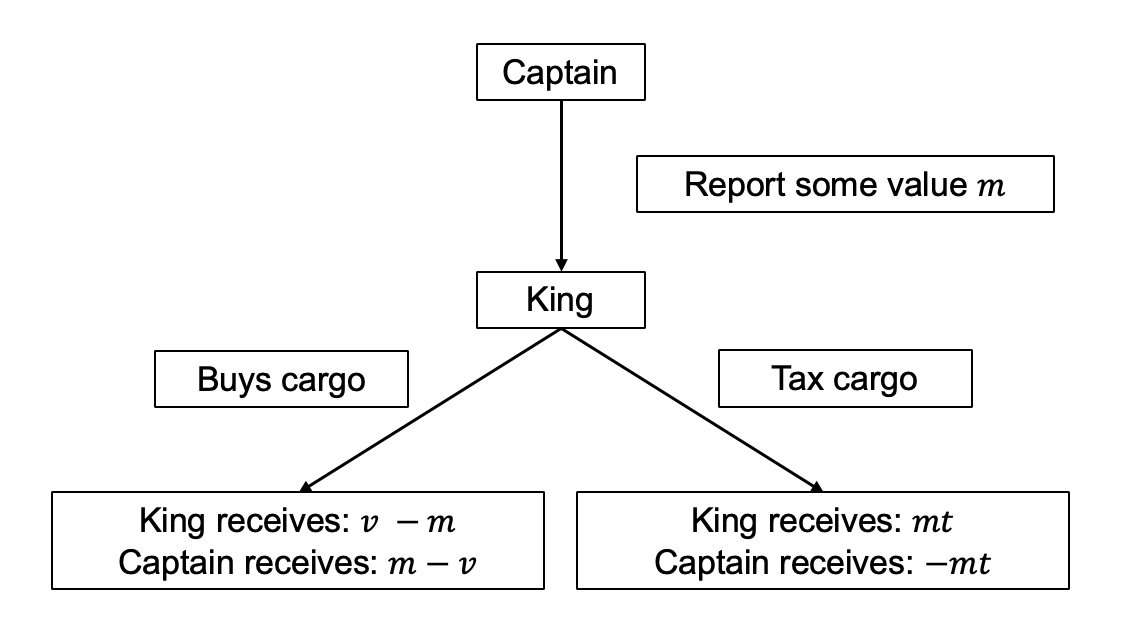
\includegraphics[width = 3.5in]{taxgamertree.png}
\end{figure}

So now we've got a model of the sound dues; let's find the strategies that the king and the capitan will play in equilibrium. Why do we care about equilibrium strategy? Well, if we're out of equilibrium, then it means that either the king or the capitan can play some other strategy to improve their outcomes. We assume that the agents would have already played an alternative strategy if there is one that improves their payoffs. With that in mind, we introduce the following theorem:

\begin{theorem}
    The king is indifferent between playing buy or tax for any equilibrium message $m$.
\end{theorem}
I will first present an intuitive proof. Suppose that the king prefers to buy the cargo. Then, knowing this, the capitan should report a higher value $m$ so that she gets paid more. She should keep on increasing the value until the king is indifferent. Similarly, suppose that the king prefers to tax the cargo, then the capitan should report a lower $m$ so she has to pay taxes, and do this until that the king is indifferent. The mathematical proof follows:
\begin{proof}
    Suppose that this isn't true and that the king strictly prefers buying the cargo. We will attempt to show a contradiction that $v - m - mt \leq 0$. Suppose that $v - (1 + t)m > 0$, then there exist some $\epsilon$ such that $m' = m + \epsilon$ and $v - (1 + t)m' > 0$. Thus, the capitan can report $m'$ instead of $m$ and gain $m'-v > m - v$, which means that $m$ is not the optimal strategy for the capitan, and thus we are not in equilibrium. The proof for when the king prefers taxing the cargo is analogous and is left as an exercise for the reader. 
\end{proof}

Given that the king is indifferent, it follows that the expected payoff that the king gets whether he buys the cargo or not is the same. That is
\begin{align*}
    v - m &= mt \\
    m &= \frac{v}{1 + t}
\end{align*}

We know that as long as the capitan plays $m = \frac{v}{1 + t}$, the king would be indifferent. We now check what the king would need to do such that the capitan would want to play $m = \frac{v}{1+t}$. Given that the king has some probability $p(m)$ of playing ``buy", the expected utility of the capitan is
\begin{align*}
    EU &= p(m)(m - v) + (1 - p(m))(-tm)
\end{align*}
The capitan gets to choose $m$, so we differentiate the equation w.r.t. $m$ and find the optimum
\begin{align*}
    \pd{EU}{m} & = p'(m)(m-v) + p(m) + p'(m)mt -t(1-p(m)) = 0 \\
    & = p'(m)m - p'(m)v + p(m) + p'(m)mt -t + tp(m) = 0
\end{align*}
We know from above that the capitan needs to play $m(1+t) = v$ for the King to be indifferent, so we can substitute that in to get
\begin{align*}
    0 & = p'(m)m - p'(m)v + p(m) + p'(m)mt -t + tp(m) \\
    & =  p'(m)m - p'(m)m(1+t)  + p(m) + p'(m)mt -t + tp(m) \\
    & = p(m) -t + tp(m) = 0
\end{align*}
Rearranging gives us
\begin{align*}
    p(m)(1 + t) & = t\\
    p(m) & = \frac{t}{1+t}
\end{align*}
In conclusion, for any given tax rate $t$, the skipper will report $m = \frac{v}{1+t}$, and the king will buy the cargo with probability $\frac{t}{1+t}$ regardless of what was reported. Here, neither player has an incentive to deviate from their current strategy, and thus we have found the Nash equilibrium of the game. 

Since the capitan will under-report the true value of their cargo, the mechanism does not induce truth-telling. We see that regardless of what the king plays he is expected to receive $\frac{t}{(1+t)}m$. Thus if the king wants to implement some tax rate $t$, he needs to find tax rate $t^*$ such that $\frac{t^*}{1+t^*} = t$.

More details on this problem can be found in \citet{Haan_2012_Taxation}, but hopefully, this small paragraph gave you a taste of how game-theoretic modeling can be applied to real life situations. 
